\documentclass[a4paper]{report}


\usepackage[italian]{babel} %italiano
\usepackage[T1]{fontenc} 
\usepackage[utf8]{inputenc}
\usepackage{graphicx} %immagini


\graphicspath{ {./img/} }

% Copyright 2017 Sergei Tikhomirov, MIT License
% https://github.com/s-tikhomirov/solidity-latex-highlighting/

\usepackage{listings, xcolor}

\definecolor{verylightgray}{rgb}{.97,.97,.97}

\lstdefinelanguage{Solidity}{
	keywords=[1]{anonymous, assembly, assert, balance, break, call, callcode, case, catch, class, constant, continue, constructor, contract, debugger, default, delegatecall, delete, do, else, emit, event, experimental, export, external, false, finally, for, function, gas, if, implements, import, in, indexed, instanceof, interface, internal, is, length, library, log0, log1, log2, log3, log4, memory, modifier, new, payable, pragma, private, protected, public, pure, push, require, return, returns, revert, selfdestruct, send, solidity, storage, struct, suicide, super, switch, then, this, throw, transfer, true, try, typeof, using, value, view, while, with, addmod, ecrecover, keccak256, mulmod, ripemd160, sha256, sha3}, % generic keywords including crypto operations
	keywordstyle=[1]\color{blue}\bfseries,
	keywords=[2]{address, bool, byte, bytes, bytes1, bytes2, bytes3, bytes4, bytes5, bytes6, bytes7, bytes8, bytes9, bytes10, bytes11, bytes12, bytes13, bytes14, bytes15, bytes16, bytes17, bytes18, bytes19, bytes20, bytes21, bytes22, bytes23, bytes24, bytes25, bytes26, bytes27, bytes28, bytes29, bytes30, bytes31, bytes32, enum, int, int8, int16, int24, int32, int40, int48, int56, int64, int72, int80, int88, int96, int104, int112, int120, int128, int136, int144, int152, int160, int168, int176, int184, int192, int200, int208, int216, int224, int232, int240, int248, int256, mapping, string, uint, uint8, uint16, uint24, uint32, uint40, uint48, uint56, uint64, uint72, uint80, uint88, uint96, uint104, uint112, uint120, uint128, uint136, uint144, uint152, uint160, uint168, uint176, uint184, uint192, uint200, uint208, uint216, uint224, uint232, uint240, uint248, uint256, var, void, ether, finney, szabo, wei, days, hours, minutes, seconds, weeks, years},	% types; money and time units
	keywordstyle=[2]\color{teal}\bfseries,
	keywords=[3]{block, blockhash, coinbase, difficulty, gaslimit, number, timestamp, msg, data, gas, sender, sig, value, now, tx, gasprice, origin},	% environment variables
	keywordstyle=[3]\color{violet}\bfseries,
	identifierstyle=\color{black},
	sensitive=false,
	comment=[l]{//},
	morecomment=[s]{/*}{*/},
	commentstyle=\color{gray}\ttfamily,
	stringstyle=\color{red}\ttfamily,
	morestring=[b]',
	morestring=[b]"
}

\lstset{
	language=Solidity,
	backgroundcolor=\color{verylightgray},
	extendedchars=true,
	basicstyle=\footnotesize\ttfamily,
	showstringspaces=false,
	showspaces=false,
	numbers=left,
	numberstyle=\footnotesize,
	numbersep=9pt,
	tabsize=2,
	breaklines=true,
	showtabs=false,
	captionpos=b
}
 %olidity color
%\begin{lstlisting}[language=Solidity]
%\end{lstlisting}

\begin{document}
\author{Giorgio Mecca}
\title{Blockchain come certificatore}
\maketitle

%abstract
\begin{abstract} 
... 
\end{abstract}

%indice
\tableofcontents

%capitolo 1
\chapter{Introduzione}
\section{Descrizione del Progetto}
\section{Descrizione dell’azienda}

%capitolo 2
\chapter{Blockchain}
\section{Problema dei generali bizantini}
\begin{figure}[h]
	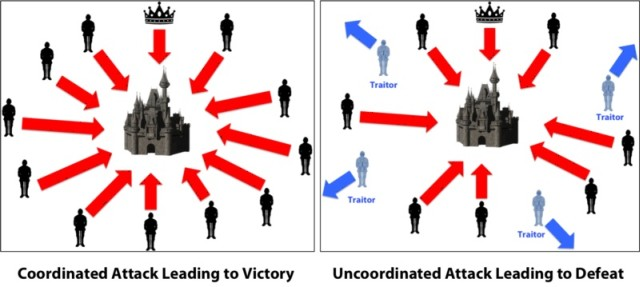
\includegraphics[width=\textwidth]{BF}
	\centering
	\caption{Problema dei generali bizantini}
	\label{fig:ByzantinFault}
\end{figure}

Il problema dei generali bizantini è un problema informatico su come raggiungere il consenso in situazioni in cui è possibile la presenza di errori. Il problema consiste nel trovare un accordo, comunicando solo tramite messaggi, tra componenti diversi nel caso in cui siano presenti informazioni discordanti. Il problema è stato teorizzato dai matematici Leslie Lamport, Marshall Pease e Robert Shostak nel 1982, i quali crearono la metafora dei generali, caso di studio molto utilizzato nei sistemi basati o che comunque utilizzano una network. La metafora si basa su diversi generali che durante un assedio sono sul punto di attaccare una città nemica. Essi sono dislocati in diverse aree strategiche e possono comunicare solo mediante messaggeri al fine di coordinare l'attacco decisivo (Figura \ref{fig:ByzantinFault}). I generali possono attaccare o ritirarsi, l'importante e che ci sia una decisione unanime, l'utilizzo di sola metà forza bellica porterebbe ad una sconfitta o una perdita. Il problema risiede quindi nell'alta probabilità che tra questi vi sia un generale traditore che mandi messaggi che vanno contro la strategia dell'esercito. La possibile soluzione punta al trovare un meccanismo secondo il quale un generale non traditore che riceva più messaggi sappia riconoscere quello veritiero. Secondo l'articolo di Lamport, Shostak e Pease non esiste una soluzione se il numero di processi non corretti è maggiore o uguale a un terzo del numero totale di processi. Una soluzione proposta è quella di Nakamoto che in una sua stesura sulla blockchain descrive un meccanisco per arrivare al consenso chiamato PoW Proof of Work.

\section{Struttura di una blockchain}
\begin{figure}[h]
	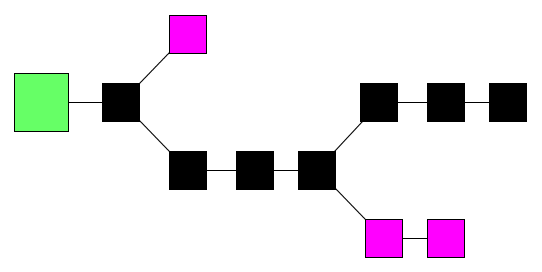
\includegraphics[width=\textwidth]{bl1}
	\centering
	\caption{Rappresentazione struttura di una blockchain}
	\label{fig:blockchain1}
\end{figure}

Una Blockchain come suggerisce l'etimologia della parola è una catena di blocchi. È una struttura dati formata da un insieme di blocchi(struttura prioritaria) collegati univocamente 1 ad 1 così da creare una metaforica catena. Una blockchain è considerata una struttura condivisa e immutabile in quanto il suo contenuto una volta scritto non è più né modificabile né eliminabile, a meno di non invalidare l'intera struttura. Questa tecnologia fà parte dei Distributed Legder cioè dei "libri mastro distribuiti" o registri condivisi infatti tutti i partecipanti della blockchain, detti anche nodi, posseggono lo stesso registro cioè le stesse informazioni andando a costruire il contrapposto di una struttura centralizzata come un Database, quindi una struttura Decentralizzata in cui ogni nodo ha la possibilità di leggere autonomamente le informazioni contenute.
Nella figura \ref{fig:blockchain1} viene visualizzata una semplice blockchain in cui sono presenti tre tipologie di blocchi quali, il blocco verde visto come il blocco di genesi, i blocchi neri che vanno a costituire la catena principale e i blocchi viola considerati blocchi orfani. L'aggiunta di un nuovo blocco è globalmente regolata da un protocollo condiviso e se autorizzata ogni nodo aggiorna la propria copia privata del registro così da evitare manipolazioni future.

\section{Hashing}
Un codice hash è una qualunque sequenza di caratteri alfanumerici generati da una particolare funzione di hash. Questa funzione prende in input un qualunque tipo di informazione e restituisce una stringa di lunghezza prefissata, questo rende la funzione one-way o non invertibile in quanto conoscendo il digest(codice hash restituito) non è possibile risalire all'informazione che lo ha generato. In una blockchain l'Hash viene utilizzato per la costruzione della catena, viene calcolato l'hash di un blocco e il blocco che lo succederà avrà come parametro questo hash. In questo modo ogni blocco è legato univocamente al blocco precedente e siccome il codice hash di un blocco viene calcolato utilizzando anche il codice hash precedente modificando un singolo blocco verrà invalidata tutta la struttura blockchain immediatamente successiva.
\begin{figure}[h]
	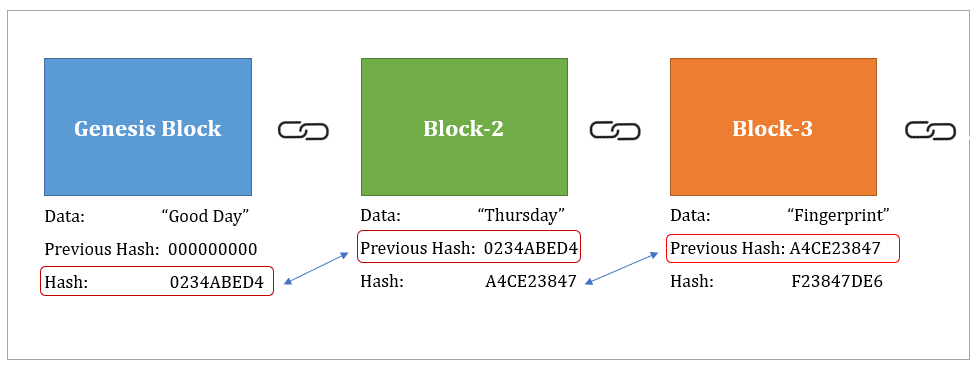
\includegraphics[width=\textwidth]{bc1}
	\centering
	\caption{Catena di una blockchain}
	\label{fig:blockchain2}
\end{figure}

\section{Transazioni}
In una blockchain i dati vengono scritti sotto forma di Transazioni in seguito contenute in vari blocchi. L'uso più comune delle transazioni è l'invio di denaro o in qualche modo una moneta equivalente. Le transazioni devono quindi avere un mittente, un destinatario e un 'value' cioè il valore trasmesso.
\section{Blocchi}
\section{Mining e Meccanismi del consenso}
\subsection{Consenso Trustless}
\subsection{Proof of Work}
\subsection{Proof of Stake}
\subsection{Proof of Authority}
\section{Attacchi}
\subsection{Selfish Mining Attack}
\subsection{Double Spending Attack}
\section{Blockchain Pubbliche/Private}
\section{Etherium}
\subsection{Smart Contract}
\subsection{Solidity}
\subsection{Gas}
\subsection{Dapps}

%capitolo 3
\chapter{Tecnologie utilizzate}
\section{Besu}
\subsection{IBFT}
\subsubsection{IBFT Methods}
\subsection{Free Gas Network}
\subsection{API Methods}
\section{Truffle}
\subsection{Compile}
\subsection{Test}
\subsection{Deploy}
\section{Node js}
\subsection{Web3}

%capitolo 4
\chapter{Caso d'uso}
\section{Problema Iniziale}
Il progetto blockchain è stato ideato e sviluppato come proposta di soluzione ai problemi nella gestione del tracciamento, invio, certificazione e mantenimento di dati riguardanti "spostamenti". Questi spostamenti sono informazioni(LOG) inviate da un qualunque ente che metta a disposizione della società o di un qualunque servizio che preveda dei mezzi pubblici o privati quali ad esempio autobus, treni, taxi etc... Queste informazioni vengono ora raccolte, analizzate e utilizzate su di modelli di storage a fogli di calcolo (Ad Esempio EXCEL - Programma Micrsoft). I fogli di calcolo offrono alcuni vantaggi come la semplicità con cui vengo creati, scritti e salvati benché offrano un'interfaccia poco user friendly('facilmente utilizzabile') guardando tutti i possibili attori, mentre il progetto si focalizza sui difetti come la pubblicazione/condivisione delle informazioni o l'interrogazione di queste in quanto utilizzando semplici fogli non vengono proposte alcune regole di struttura e organizzazione,e ci si pone particolare importanza alla sicurezza e all'affidabilità di queste informazioni e che non vengano modificate durante la condivisione, quindi la possibile certificazione di essi.

\section{Soluzione}
La soluzione proposta si offre di risolvere tutti i problemi sopra elencati come la certificazione, salvataggio e interrogazioni di informazioni. Viene ideata una blockchain privata che avrà funzione di ente (decentralizzato) certificatore, questa non utilizza nessuna moneta creando una Free Gas Network e che con l'ausilio di appositi smart contract(scritti e caricati autonomamente) ci permette di salvare un codice che andrà ad identificare un determinato gruppo di spostamenti come un codice Hash che usufruendo della struttura e utilizzo della blockchain non potrà essere modificato, ciò implica che si potrà sempre verificare la correttezza del gruppo di spostamenti richiesti ricreando e controllando il loro codice.

La memorizzazione dei dati viene invece affidata ad un database relazionale, utilizzando nel progetto il DBMS(DataBase Managenent System) MySql, che ci permette di salvare grandi quantità di dati con una efficiente organizzazione gestita con la creazione di tabelle così da essere facilmente interrogabile in futuro.
 
L'interfaccia comune è gestita con un server sviluppato tramite tecnologia node js che con una single Page Application avrà la funzione di interfaccia user friendy con funzioni di memorizzazione per i log degli spostamenti su Database, calcolo e salvataggio dei loro codici hash sulla blockchain al tempo stimato e quando necessario, cioè quando e ovunque verranno richiesti dei dati e avverrà l'interrogazione del DataBase sarà reso obbligatorio il controllo di questi con il codice sulla blockchain. Inserendo questo WebServer intermedio o server proxy si andrà ad eliminare il passaggio di dati non propriamente protetto e rende partecipi tutti i singoli attori dell'attività.

\subsection{Problematiche}
Utilizzando delle nuove tecnologie sorgono comunque nuove problematiche che non sono state affrontate nello sviluppo in quanto non inerenti ai fini del progetto.

%DOS utilizzando un solo server
Una prima problematica si sviluppa utilizzano un server proxy. Avendo un singolo server di accesso al database a alla blockchain sequesto non viene correttamente protetto e costantemente controllato è soggetto ai classici attacchi come un DDOS - Distributed Denial of Service in cui si utilizzano molteplici messaggi fittizi (come un inizio di HandShake per una connessione TCP) per far si che il server non possa sostenere tutti i servizi e essendo l'unico punto di accesso bloccherebbe  l'intero accesso alla rete blockchain.

%blockchain utile solo con molti nodi
Una caratteristica che rende sicura la blockchain pubblica è la molteplicità di nodi, questa con una blockchain privata come la nostra va a decadere con il discendere  del numero di nodi; utilizzando un meccanisco di conseso basato su PoA(Proof of Autority) si ha infatti bisogno di un minimo di 4 nodi per essere resistente al problema bizantino.

%attacco del compleanno
Per evitare l'appesantimento della Blockchain si è pensato di salvare su di essa solo un codice identificativo(codice Hash) per un gruppo di Log. Questo implica che con l'aumentare dei log identificati da un singolo codice hash diminuisca la sicurezza che questo apporta infatti sarà più facilmente utilizzabile un attacco come l'attacco del compleanno che ha come obiettivo quello di generare una collisione cioè di trovare dei dati fittizi ai Log originari che però generano lo stesso codice Hash, questi dati fittizi potranno essere quindi sostituiti nel DB ma verranno comunque considerati certificati dal sistema in quanto produrranno lo stesso codice.

\section{Attori}
Il caso d'uso per il progetto blockchain prevede la partecipazione di diversi attori quali: 

Un Terminal User o utente finale è un comune dipendente di un ente che partecipa alla blockchain il quale ha il compito di comunicare i propri spostamenti/Log o qualunque informazione di cui si preveda il salvataggio;

Gli Admin sono dei dipendenti di enti partecipanti che vengono segnati dagli stessi come amministratori che quindi posseggono  particolari oneri come il possesso e la trasmissione di una chiave privata;

Il proprietario/gestore della blockchain avrà il compito di gestire l'intera blockchain privata con l'amministrazione che ne segue, come la supervisione dei nodi presenti, il loro funzionamento e la loro caratterizzazione come validatori. 
\section{Scenario di utilizzo}
Il Progetto prevede uno scenario di utilizzo diverso seguendo la distinzione degli attori.
Per l'utilizzo si prevede che ad ogni ente partecipante al progetto gli venga assegnato un account, cioè una copia di chiavi privata e pubblica che serviranno per interagire con la blockchain, inoltre ogni ente dovrà inserire i propri dipendenti nel Database e specificare il ruolo di essi, se admin o Terminal User.

Un Terminal User, una volta effettuato l'accesso, viene portato ad un'interfaccia in cui può inserire la città che sarà selezionata come Start dello spostamento e in seguito viene spostato in una seconda interfaccia da cui può terminare lo spostamento o annullarlo, se annullato potrà cominciare un nuovo spostamento dalla precedente interfaccia, il completamento di questo avverrà solo se compila i campi necessari quali la città di Termine e la distanza percorsa indicata in Kilometri.

Un admin, una volta effettuato l'accesso, potrà a differenza di un Terminal User effettuare delle query/ interrogazioni riguardo gli spostamenti compiuti, inserendo una data otterrà tutti gli spostamenti che sono stati certificati da una transazione inserita in quella determinata data, da qui potrà anche accedere ai dettagli della transazione o del blocco che la contiene riferendoci alla blockchain, inoltre, quando il sistema lo richiede, ha il compito di inserire la Private Key dell'utente(ente) che verrà utilizzata per la scrittura su blockchain.

%capitolo 5
\chapter{Sviluppo}
\section{Schema Progetto}
\section{Blockchain Ibrida}
\section{Smart Contract}
\subsection{Boxing}
\section{WebApp}
\subsection{Single Page Application}
\subsection{Input}
\subsubsection{Inserimento in un DB}
\subsubsection{Inserimento nella Blockchain}
\subsection{Output}
\subsubsection{Report di Controllo}
\subsubsection{Monitor Blockchain}

%capitolo 6
\chapter{Sviluppi futuri}
\section{Analisi costi}
\section{Immissione nella blockchain pubblica}
\section{Blockchain pubblica come certificazione}
\section{Svilupo full Blockchain}


%lista delle Immagini
\listoffigures

\end{document}
